\documentclass{beamer}

\usepackage[utf8]{inputenc}
\usepackage[ngerman]{babel}

\mode<presentation> {
  %\setbeameroption{show notes} % Kommentare im fertigen PDF

  \usetheme{Boadilla}
  \usecolortheme{seagull}

  \setbeamertemplate{footline}[page number] % Einfacher Folienzähler als Fußzeile
  \setbeamertemplate{navigation symbols}{} % Keine Navigationslinks
}

\title[Frank]{Frank -- eine Programmiersprache mit Effekten}
\author{Tim Baumann}
\institute[CCA]{Curry Club Augsburg}
\date{23. Februar 2017}

\usepackage[outputdir=output]{minted} % Syntax-Highlighted Code; requires pygments to be installed
\newminted[frankcode]{agda}{}
\newmintinline[frankinline]{haskell}{}

\usepackage{hyperref}
\usepackage{graphicx}

\begin{document}

\begin{frame}
  \titlepage
\end{frame}

\begin{frame}
  \begin{tabular}{r l}
    Paper: &
      \href{https://arxiv.org/abs/1611.09259}{Do Be Do Be Do} \\
      & von Sam Lindley, Conor McBride und Craig McLaughlin \\

    GitHub: & \url{https://github.com/cmcl/frankjnr} \\
  \end{tabular}
\end{frame}

\begin{frame}
  \begin{center}
    \huge
    "`To be is to do"' -- Socrates \\
    "`To do is to be"' -- Sartre \\
    "`Do Be Do Be Do"' -- Sinatra

    \vspace{1cm}
    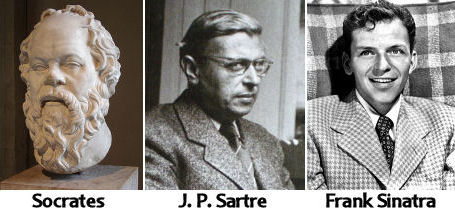
\includegraphics[width=8cm]{socratessartresinatra}
  \end{center}
\end{frame}

\begin{frame}
  \frametitle{Berechnungen und Werte}

  Grundprinzip in Frank: Es werden
  \begin{itemize}
    \item Werte, die \textit{sind}, und
    \item Berechnungen, die \textit{tuen},
  \end{itemize}
  voneinander getrennt.
\end{frame}

\begin{frame}[fragile]
  \frametitle{Berechnungen und Werte}

\begin{frankcode}
data List X = nil | cons X (List X)

map : {{X -> Y} -> List X -> List Y}
map f nil         = nil
map f (cons x xs) = cons (f x) (map f xs)
\end{frankcode}

\begin{itemize}
  \item<2-> Regel: Typen von Berechnungen sind von der Form \frankinline{{t1 -> ... -> tn -> r}} mit null oder mehr Argumenten.
  \item<3-> Berechnungen werden unausgewertet übergeben, Werte ausgewertet übergeben. Argumente werden in der Reihenfolge von links nach rechts ausgewertet.
  \item<4-> Berechnungen mit Argumenten führt man aus, indem man Argumente übergibt
  \item<5-> 
    Etwas Syntaxzucker: Wir werden die ganz äußeren Klammern bei Funktionsdefinitionen weglassen:

    \begin{frankcode}
    map : {X -> Y} -> List X -> List Y
    \end{frankcode}
\end{itemize}
\end{frame}

\begin{frame}[fragile]
  \frametitle{Berechnungen und Werte}

\begin{frankcode}
data Bool = tt | ff

if : Bool -> {X} -> {X} -> X
if tt t _ = t!
if ff _ f = f!
\end{frankcode}

\begin{itemize}
  \item<2-> Regel: Eine nullstellige Berechnung \frankinline{f : {X}} führt man mit einem Ausrufezeichen aus: \frankinline{f! : X}
\end{itemize}

\begin{visibleenv}<3->
\begin{frankcode}
if fire! {launch missiles} {unit}
\end{frankcode}
\end{visibleenv}

\begin{itemize}
  \item<4-> Regel: Ist \frankinline{x : X} ein Wert, so ist \frankinline{{x} : {X}} die Berechnung, die diesen Wert produziert.
\end{itemize}

\end{frame}

\begin{frame}[fragile]
  \frametitle{Berechnungen und Werte}

Man kann Case-Style-Pattern-Matching in der Sprache definieren:

\begin{frankcode}
on : X -> {X -> Y} -> Y
on x f = f x

shortAnd : Bool -> {Bool} -> Bool
shortAnd x c = on x { tt -> c! | ff -> ff }
\end{frankcode}
\end{frame}

\begin{frame}[fragile]
  \frametitle{Effekte}

\begin{frankcode}
interface Send X = send : X -> Unit 

interface Receive X = receive : X

chatbot : {[Send String, Receive String]Unit}
chatbot! =
  send "Hallo! Wie heißt du?";
  send ("'" ++ receive! ++ "' ist ein schöner Name!");
  chatbot!
\end{frankcode}

\begin{onlyenv}<1>
\begin{frankcode}
data Unit = unit

(;) : X -> Y -> Y
(;) x y = y
\end{frankcode}
\end{onlyenv}

\begin{onlyenv}<2->
\begin{itemize}
  \item<2-> Regel: Jede Berechnung, die Interfaces verwendet, muss diese in eckigen Klammern vor dem Rückgabetyp angeben:
  \frankinline{{t1 -> ... -> tn -> [I1, ..., Im]}}
\end{itemize}
\end{onlyenv}
\end{frame}

\begin{frame}[fragile]
  \frametitle{Effekte}

\begin{frankcode}
data Void =

interface Abort = aborting : Void

abort : [Abort]X
abort! = on aborting! {}
\end{frankcode}
\end{frame}

\begin{frame}[fragile]
  \frametitle{Effekte}

\begin{frankcode}
interface State S = get : S
                  | put : S -> Unit

next : [State Int]Int
next! = fst get! (put (get! + 1))

fst : X -> Y -> X
fst x y = x
\end{frankcode}
\end{frame}

\begin{frame}[fragile]
  \frametitle{Effekte}

\begin{frankcode}
sends : List X -> [Send X]Unit
sends xs = map send xs; unit

indexer : List X -> [State Int]List (X, Int)
indexer xs = map {x -> (x, next!)} xs

-- map : {X ->   Y} -> List X ->   List Y
-- map : {X -> []Y} -> List X -> []List Y
\end{frankcode}

\begin{itemize}
  \item<2->
    Regel: Jede Berechnung ist implizit polymorph in ihren Effekten.
    Man kann \frankinline{map} mit einer Berechnung, die das \frankinline{Send}-Interface verwendet, als Argument aufrufen.
    Das Ergebnis ist eine Berechnung, die ebenfalls das \frankinline{Send}-Interface verwendet.
\end{itemize}
\end{frame}

\begin{frame}[fragile]
  \frametitle{Effekt-Handler}

\begin{frankcode}
state : S -> <State S>X -> X
state _ x            = x
state s <get -> k>   = state s (k s)
  -- k : X -> <State S>X
state _ <put s -> k> = state s (k unit)
  -- k : Unit -> <State S>X
\end{frankcode}

\begin{itemize}
  \item<2->
    Regel: Jede Berechnung hat die Möglichkeit, die Effekte ihrer übergebenen Berechnungen zu behandeln.
    Im Typ werden die behandelten Interfaces in eckigen Klammern angegeben.
\end{itemize}

\begin{visibleenv}<3->
\begin{frankcode}
index : List X -> List (X, Int)
index xs = state 0 (indexer xs)
  -- indexer : List X -> [State Int]List (X, Int)
  -- e.g. index "abc" == [('a', 0), ('b', 1), ('c', 2)]
\end{frankcode}
\end{visibleenv}

\end{frame}

\begin{frame}[fragile]
  \frametitle{Effekt-Handler}

\begin{frankcode}
catch : <Abort>X -> {X} -> X
catch x               _ = x
catch <aborting -> _> f = f!
\end{frankcode}

\end{frame}

\begin{frame}[fragile]
  \frametitle{Effekt-Handler}

\begin{frankcode}
feed : List R -> <Receive R>X -> [Abort]X
feed _           x              = x
feed (cons x xs) <receive -> k> = feed xs (k x)
feed nil         <receive -> _> = abort!
\end{frankcode}

\end{frame}

\begin{frame}[fragile]
  \frametitle{Effekt-Handler}

\begin{frankcode}
pipe : <Send X>Unit -> <Receive X>Y -> [Abort]Y
pipe <send x -> s> <receive -> r> = pipe (s unit) (r x)
pipe _             y              = y
pipe <_>           y              = y
pipe unit          <_>            = abort!
\end{frankcode}

\end{frame}

\begin{frame}[fragile]

\begin{frankcode}
spacer : [Send String, Receive String]Unit
spacer! = send receive!; send " "; spacer!

catter : [Receive (List X)]List X
catter! =
  on receive!
    { nil -> nil
    | xs  -> xs ++ catter!
    }

pipe
  (sends ["do", "be", "do", ""])
  (pipe spacer! catter!)
-- evaluates to ["do", " ", "be", " ", "do", ""]
\end{frankcode}

\end{frame}

\begin{frame}[fragile]

\begin{frankcode}
interface Choice = choice : Bool

data Toss = Heads | Tails

toss : [Choice]Toss
toss! = if choice! {Heads} {Tails}

drunkToss : [Choice, Abort]Toss
drunkToss! = if choice! toss abort

drunkTosses : Int -> [Choice, Abort]List Toss
drunkTosses 0 = nil
drunkTosses n = cons drunkToss! (drunkTosses (n-1))

\end{frankcode}

\end{frame}

\begin{frame}[fragile]

\begin{frankcode}
allChoices : <Choice>X -> List X
allChoices x             = cons x nil
allChoices <choice -> k> =
  allChoices (k true) ++ allChoices (k false)

data Maybe X = nothing | just X

maybeAbort : <Abort>X -> Maybe X
maybeAbort x               = just x
maybeAbort <aborting -> k> = nothing
\end{frankcode}

\begin{frankcode}
t5 : Maybe (List (List Toss))
t5! = maybeAbort (allChoices (drunkTosses 2))
\end{frankcode}

\begin{visibleenv}<2->
\begin{frankcode}
-- nothing
\end{frankcode}
\end{visibleenv}

\begin{frankcode}
t6 : List (Maybe (List Toss))
t6! = allChoices (maybeAbort (drunkTosses 2))
\end{frankcode}

\begin{visibleenv}<2->
\begin{frankcode}
-- [just [Heads, Heads], just [Heads, Tails], nothing,
--  just [Tails, Heads], just [Tails, Tails], nothing, nothing]
\end{frankcode}
\end{visibleenv}

\end{frame}

\end{document}